
\section{Nekomutativen Choquetov rob}\label{sec:12}

V tem poglavju definiramo Arvesonove robne upodobitve (\cite{arveson1969}), ki predstavljajo nekomutativno posplošitev točk v Choquetovem robu za operatorske sisteme v $C(X)$.
Dokazali bomo, da za vsak operatorski sistem $\mathcal{S}$ obstaja dovolj robnih upodobitev, da {povsem normirajo} $\mathcal{S}$.
Pri tem sledimo članku Davidsona in Kennedyja \cite{davidson2015},
v katerem avtorja posplošita argumente Arveson-Dritschel-McColloughovega izreka za obstoj čistih maksimalnih dilatacij.

Kot v prejšnjem poglavju tudi tokrat najprej začnemo z operatorskim sistemom $\mathcal{S} \subseteq C(X)$,
ki loči točke na $X$.
V tem kontekstu pravimo, da regularna Borelova verjetnostna mera (od sedaj naprej le: verjetnostna mera) $\mu$ na $X$ \emph{zastopa} točko $x \in X$,
če velja $$f(x) = \int_X f\, d\mu,\quad \forall f \in \mathcal{S}.$$
Takoj je očitno, da vsako točko $x \in X$ zastopa njena Diracova delta $\delta_x$.

\begin{definicija}
    Naj bo $\mathcal{S} \subseteq C(X)$ operatorski sistem, ki loči točke na $X$.
    \emph{Choquetov rob} $\mathcal{S}$ je množica vseh točk $x \in X$,
    za katere je Diracova delta $\delta_x$ edina verjetnostna mera, ki jih zastopa.
\end{definicija}


\begin{zgled}
    Vrnimo se k operatorskemu sistem
    $$\mathcal{S} = \C [z] + \C[z]^* \subseteq C(\overline{\D}).$$
    Dokazujemo, da je tudi njegov Choquetov rob enak $\T$.

    Vzemimo poljubno točko $\lambda \in \T$ in naj bo $\mu$ verjetnostna mera, ki jo zastopa.
    Potem je $$2 = \left| \int_{\overline{\D}} (z + \lambda)\, d\mu \right| \leq \int_{\overline{\D}} \left| z + \lambda\right| \, d\mu \leq 2,$$
    torej je $\int_{\overline{\D}} (2 - |z + \lambda|)\, d\mu = 0$ in $2 = | z + \lambda|$ $\mu$-skoraj povsod na $\overline{\D}$.
    Ker velja $2 - |z + \lambda| = 0$ samo za $z = \lambda$, to pomeni, da je $\mu (\{\lambda\}) = 1$.
    Slednje implicira, da je $\mu = \delta_\lambda$.

    Dokažimo še, da poljubna točka $\lambda \in {\D}$ ni v Choquetovem robu.    
    Definiramo Poissonovo jedro za $\overline{\D}$
    $$P(\lambda, z) = \frac{1 - |\lambda|^2}{|z - \lambda|^2},\quad z \in \T.$$
    Znano dejstvo je (glej na primer \cite[Theorem 15, str. 41]{evans2010}), da za vsako realno harmonično funkcijo $g$ na $\D$, ki je zvezna na $\overline{\D}$, 
    velja Poissonova reprezentacijska formula
    $$g(\lambda) = \int_{\T} g(z) P(\lambda, z)\, dm ,$$
    pri čemer je $m$ normalizirana Lebesgueova mera na $\T$. 
    Opazimo, da lahko vsako funkcijo $f \in \mathcal{S}$ zapišemo kot $f(x, y) = p(x, y) + i q(x, y)$,
    kjer sta $p, q$ realna polinoma (in zato harmonični funkciji na $\D$). To pomeni, da je 
    \begin{align*}
        f(\lambda) &= p(\lambda) + i q(\lambda) \\
        &= \int_{\T} p(z) P(\lambda, z)\, dm + i \int_{\T} q(z) P(\lambda, z)\, dm \\ 
        &= \int_{\T} (p(z) + i q(z)) P(\lambda, z)\, dm \\ 
        &= \int_{\T} f(z) P(\lambda, z)\, dm.
    \end{align*}
    Definiramo sedaj mero $\omega_\lambda$ na $\overline{\D}$,
    tako da je za vsako Borelovo množico $E \subseteq \overline{\D}$ 
    $$\omega_\lambda (E) := \int_{E \cap \T} P(\lambda, z)\, dm (z).$$ Potem je $\omega_\lambda$
    verjetnostna mera na $\overline{\D}$, tako da velja 
    $$f(\lambda) = \int_{\overline{\D}} f\, d\omega_\lambda$$
    za vse $f \in \mathcal{S}$. Ker je $\omega_\lambda \neq \delta_\lambda$,
    točka $\lambda$ ni v Choquetovem robu.

    Opazimo lahko, da rob Šilova in Choqueta za operatorski sistem $\mathcal{S}$ sovpadata. 
    Kot bomo videli kasneje, to ni naključje.
\end{zgled}

Če želimo definicijo Choquetovega robu prenesti na splošne operatorske sisteme,
jo moramo najprej prevesti v jezik funkcionalne analize.
Za poljubno točko $x \in X$ lahko definiramo $*$-homomorfizem 
$$\ev_x: C(X) \to \C,\quad f \mapsto f(x).$$
Ker po Rieszovem reprezentacijskem izreku vsakemu enotskemu pozitivnemu funkcionalu na $C(X)$
ustreza enolično določena verjetnostna mera na $X$, 
je vsaka točka $x \in X$ v Choquetovem robu natanko tedaj, ko ima funkcional $\ev_x |_{\mathcal{S}}: \mathcal{S} \to \C$
enolično pozitivno razširitev do $C(X)$.
Od tod takoj sledi naslednja trditev.

\begin{trditev}
    Choquetov rob $\mathcal{S}$ sestavljajo natanko točke $x \in X$, za katere ima $\ev_x |_{\mathcal{S}}$ lastnost enolične preslikave.
\end{trditev}


Preostane še najti primeren nekomutativen analog preslikavam $\ev_x :C(X) \to \C$ za $x \in X$.
Ta analog bodo \emph{nerazcepne upodobitve}. To so upodobitve $C^*$-algeber $\pi: \mathfrak{A} \to \bh$,
ki nimajo nobenega netrivialnega zaprtega invariantnega podprostora v $\mathcal{H}$.
Po standardnem izreku iz funkcionalne analize (\cite[Theorem 5.1.5., str. 143]{murphy1990}) je slednji pogoj ekvivalenten $\pi(\mathfrak{A}) ' = \C \cdot I_{\mathcal{H}}$.
Ni težko videti, da je preslikava $\ev_x: C(X) \to \C$ nerazcepna upodobitev $C^*$-algebre $C(X)$ za poljubno točko $x \in X$.
Velja pa tudi obratno.

\begin{trditev}
    Vsaka nerazcepna upodobitev $C(X)$ je oblike $\ev_x : C(X) \to \C$
    za neko točko $x \in X$.
\end{trditev}

\begin{dokaz}
    Naj bo $\rho: C(X) \to \bh$ nerazcepna upodobitev, torej $\rho(C(X))' = \C \cdot I_{\mathcal{H}}$.
    Ker je $C(X)$ komutativna algebra, je tudi $\rho(C(X))$ komutativna algebra in v posebnem velja 
    $\rho(C(X)) \subseteq \rho(C(X))' = \C \cdot I_{\mathcal{H}}$. To pomeni, da je vsak podprostor v $\mathcal{H}$
    invarianten za $\rho$, zato mora biti $\dim \mathcal{H} = 1$ in lahko vzamemo $\mathcal{H} \equiv \C$.
    To pomeni, da je $\rho: C(X) \to \mathcal{B}(\C) \equiv \C$ multiplikativen funkcional.

    Naprej dokazujemo, da je njegovo jedro $\ker \rho$ maksimalen ideal v $C(X)$. Vzemimo poljuben ideal $\ker \rho \subsetneqq I \subseteq C(X)$,
    tako da obstaja $f \in I \setminus \ker \rho$, za katerega velja $\rho(f) \neq 0$ in $1 - \frac{f}{\rho(f)} \in \ker \rho$.
    Od tod sledi $$1 = \left(1 - \frac{f}{\rho(f)}\right) + \frac{1}{\rho(f)} \cdot f \in I,$$
    zato je $I = C(X)$ in $\ker \rho$ je maksimalen (zaprt) ideal v $C(X)$.
    
    Po korespondenci med zaprtimi ideali v $C(X)$ in zaprtimi množicami v $X$ obstaja neka točka $x \in X$,
    tako da je $\ker \rho = I(\{x\})$. Potem za poljubno funkcijo $f \in C(X)$ velja
    $f - f(x) \cdot 1 \in \ker \rho$, od koder sledi 
    $$\rho(f) - f(x) = 0$$
    in $\rho = \ev_x$.
\end{dokaz}

Zadnji dve trditvi motivirata naslednjo definicijo.

\begin{definicija}
    \emph{Robna upodobitev} operatorskega sistema $\mathcal{S} \subseteq C^*(\mathcal{S})$ je nerazcepna upodobitev $\rho: C^*(\mathcal{S}) \to \bh$,
    tako da ima $\rho|_{\mathcal{S}}$ lastnost enolične razširitve.
\end{definicija}

Dokazali smo že, da so robne upodobitve za operatorski sistem $\mathcal{S} \subseteq C^*(\mathcal{S}) = C(X)$
sovpadajo s preslikavami $\ev_x$ za točke $x$ v Choquetovem robu. Vendar pa za splošen operatorski sistem
iz definicije ni takoj očitno, da robne upodobitve sploh obstajajo. V tem poglavju bomo dokazali, da za poljuben operatorski sistem $\mathcal{S} \subseteq C^*(\mathcal{S})$
obstaja dovolj robnih upodobitev, da \emph{povsem normirajo} $\mathcal{S}$: to pomeni,
da za vsako matriko $A \in M_n (\mathcal{S})$ obstaja robna upodobitev $\varphi$, tako da je $\| \varphi^{(n)} (A)\| = \| A\|$.

Najprej uvedemo nov pojem.

\begin{definicija}
    Preslikava $\varphi \in \PP (\mathcal{S}, \bh)$ je \emph{čista},
    če je vsak $\psi \in \PP (\mathcal{S}, \bh)$, za katerega velja $0 \leq \psi \leq \varphi$,
    oblike $\psi =  t \varphi$ za nek $0 \leq t \leq 1$.
\end{definicija}

\begin{zgled}
    Oglejmo si množico stanj 
    $$S(\mathcal{S}) = \{\omega \in \mathcal{S}^*\ |\ \text{$\omega$ pozitiven}, \| \omega\| = 1 \}$$ 
    na operatorskem sistemu $\mathcal{S}$. Potem je $S(\mathcal{S})$ neprazna, konveksna 
    in po Banach-Alaoglujevem izreku kompaktna v šibki-$*$ topologiji.
    Po Krein-Milmanovem izreku \cite[Theorem V.7.4., str. 142]{conway1990} ima zato neprazno množico ekstremnih točk, ki jo označujemo z $\ext S(\mathcal{S})$.
    Dokazujemo, da je stanje na $\mathcal{S}$ čisto natanko tedaj, ko je element $\ext S(\mathcal{S})$
    (slednje običajno vzamemo za definicijo čistih stanj).

    Denimo najprej, da stanje $\omega$ ni v $\ext S(\mathcal{S})$, torej obstajata $\omega_1, \omega_2 \in S(\mathcal{S})$, ki nista enaka $\omega$ in za katera velja
    $\omega = \frac{1}{2} \omega_1 + \frac{1}{2} \omega_2$. Potem je $0 \leq \frac{1}{2} \omega_1 \leq \omega$,
    vendar pa $\frac{1}{2} \omega_1$ ni skalarni večkratnik $\omega$. 
    
    V obratno smer predpostavimo, da obstaja pozitiven funkcional $\psi$,
    ki ni skalarni večkratnik $\omega$ in velja $0 \leq \psi \leq \omega$. Potem označimo $t = \psi(1)$
    in definiramo stanji $\omega_1 := \frac{1}{t} \psi$ ter $\omega_2 := \frac{1}{1 - t} (\omega - \psi)$, ki nista enaki $\omega$.
    Potem je $\omega = \frac{1}{2} \omega_1 + \frac{1}{2} \omega_2$, torej ne more biti čisto stanje.
\end{zgled}

Razlog za vpeljavo čistih preslikav je naslednja karakterizacija Choquetovega robu (\cite[Proposition 6.2, str. 29]{phelps2001}):
\emph{če je $\mathcal{S} \subseteq C(X)$ operatorski sistem, ki loči točke na $X$,
potem je točka $x \in X$ v Choquetovem robu natanko tedaj, ko je $\ev_x$ čisto stanje}.
V nadaljevanju bomo potrebovali različico te ekvivalence za splošne operatorske sisteme.

\begin{trditev}\label{trd:aux2}
    Naj bo $\mathcal{S} \subseteq C^* (\mathcal{S})$ operatorski sistem in $\rho: C^*(\mathcal{S}) \to \bh$
    upodobitev. Potem je $\rho$ robna upodobitev za $\mathcal{S}$ natanko tedaj, ko je $\varphi|_{\mathcal{S}}: \mathcal{S} \to \bh$
    čista in maksimalna.
%    Če je enotska povsem pozitivna preslikava $\varphi: \mathcal{S} \to \bh$ čista in maksimalna, potem je njena enolična razširitev 
%    $\rho: C^* (\mathcal{S}) \to \bh$ robna upodobitev.
\end{trditev}

Za dokaz potrebujemo naslednjo lemo.

\begin{lema}
    Naj bo $\mathfrak{A}$ $C^*$-algebra.
    Preslikava $\varphi \in \PP (\mathfrak{A}, \bh)$ je {čista} natanko tedaj, ko ima 
    njena minimalna Stinespringova upodobitev $(\pi, V, \mathcal{K})$ nerazcepno upodobitev $\pi$.
\end{lema}

\begin{dokaz}
    Po trditvi \ref{trd:1.4} imamo bijektivno korespondenco med množicama 
    $$\{\psi \in \PP (\mathfrak{A}, \bh)\ |\ 0 \leq \psi \leq \varphi\}$$
    ter $$\{T \in \pi(\mathfrak{A})'\ |\ 0 \leq T \leq I\}.$$
    Slednja množica vsebuje skalarje natanko tedaj, ko je $\pi(\mathfrak{A})' = \C \cdot I$.
\end{dokaz}

\begin{dokaz}[Dokaz trditve \ref{trd:aux2}]
    Najprej predpostavimo, da je $\rho|_{\mathcal{S}}$ čista in maksimalna.
    Dovolj je dokazati, da je $\rho$ nerazcepna upodobitev.
    Denimo nasprotno, torej obstaja nek Hilbertov podprostor $(0) \lneqq \mathcal{K} \lneqq \mathcal{H}$,
    ki reducira $\rho$. Naj bo $P \in \bh$ ortogonalna projekcija na $\mathcal{K}$, torej $P \in \rho(C^* (\mathcal{S}))'$.
    Potem je $\varphi := P \rho$ povsem pozitivna preslikava in $0 \leq \varphi|_{\mathcal{S}} \leq \rho|_{\mathcal{S}}$.
    Ker pa $\varphi (1) = P$ ni skalar, smo prišli v protislovje s tem, da je $\rho|_{\mathcal{S}}$ čista.

    Sedaj dokažimo še nasprotno. Denimo, da je $\rho: C^*(\mathcal{S}) \to \bh$ robna upodobitev.
    Ker je $\rho$ upodobitev, je sama svoja minimalna Stinespringova upodobitev, in ker je nerazcepna,
    je po prejšnji lemi tudi čista preslikava. Zadošča dokazati, da je potem tudi $\rho|_{\mathcal{S}}: \mathcal{S} \to \bh$
    čista preslikava. Denimo nasprotno, torej obstajata $\varphi_1, \varphi_2 \in \PP(\mathcal{S}, \bh)$, ki nista skalarna večkratnika $\rho|_{\mathcal{S}}$
    in za katera velja $\rho|_{\mathcal{S}} = \varphi_1 + \varphi_2$.
    Po Arvesonovem razširitvenem izreku ju lahko razširimo do povsem pozitivnih preslikav $\psi_1, \psi_2 \in \PP(C^*(\mathcal{S}), \bh)$.
    Ker ima $\rho|_{\mathcal{S}}$ lastnost enolične preslikave, je $\rho = \psi_1 + \psi_2$.
    Ker je $0 \leq \psi_1 \leq \rho$, smo v protislovju s tem, da je $\rho$ čista preslikava.
\end{dokaz}

Trditev \ref{trd:aux2} nam pove, da lahko vsako čisto maksimalno preslikavo na operatorskem sistemu $\mathcal{S}$ razširimo do robne upodobitve.
Preostane nam še, da konstruiramo čiste maksimalne preslikave. To bomo naredili na podoben način, kot v poglavju o $C^*$-algebrah,
v katerem smo konstruirali maksimalne dilatacije.
Naslednji izrek je analog Arveson-Dritschel-McColloughovega izreka za čiste preslikave.

\begin{izrek}[Davidson-Kennedy]\label{izr:3.1}
    Vsako čisto enotsko povsem pozitivno preslikavo $\varphi: \mathcal{S} \to \mathcal{B}(\mathcal{H})$ lahko dilatiramo do maksimalne čiste preslikave
    $\psi: \mathcal{S} \to \mathcal{B}(\mathcal{K})$, ki ima razširitev na robno upodobitev.
\end{izrek}

Pri dokazu bomo uporabili skoraj enake argumente kot pri dokazu izreka \ref{izr:2.2},
le da bodo sedaj dilatacije čiste. Spomnimo se leme \ref{lem:2.1}, ki pravi, da za vsako 
usmerjeno množico enotskih povsem pozitivnih preslikav $\{\varphi_{\lambda} : \mathcal{S} \to \mathcal{B} (\mathcal{H}_\lambda)\}_{\lambda \in \Lambda}$ 
z relacijo $\preceq$ obstaja enolično določena enotska povsem pozitivna preslikava $\varphi_{\infty}: \mathcal{S} \to \mathcal{B} (\mathcal{H}_\infty)$,
tako da je $\varphi_\infty \succeq \varphi_{\lambda}$ za vsak $\lambda \in \Lambda$. 

Naslednja lema je njen analog za čiste dilatacije.

\begin{lema}
    Naj bo $\{\varphi_{\lambda} : \mathcal{S} \to \mathcal{B} (\mathcal{H}_\lambda)\}_{\lambda \in \Lambda}$ 
    usmerjena množica čistih enotskih povsem pozitivnih preslikav z relacijo $\preceq$.
    Definirajmo $\mathcal{H}_\infty$ kot napolnitev prostora $\bigcup_{\lambda \in \Lambda} \mathcal{H}_\lambda$.
    Potem obstaja čista enolično določena preslikava $\varphi_{\infty} \in \EPP (\mathcal{S}, \mathcal{B} (\mathcal{H}_\infty))$,
    tako da je $\varphi_\infty \succeq \varphi_{\lambda}$ za vsak $\lambda \in \Lambda$. 
\end{lema}

\begin{dokaz}
    Obstoj in enoličnost dilatacije $\varphi_\infty$ že imamo po lemi \ref{lem:2.1}.
    Dokazati moramo le, da je $\varphi_\infty$ tudi čista preslikava.
    Vzemimo poljubno $\psi \in \PP (\mathcal{S}, \mathcal{B}(\mathcal{H}_\infty))$, 
    za katero velja $0 \leq \psi \leq \varphi_\infty$. Potem za vsak $\lambda \in \Lambda$ velja $0 \leq P_{\mathcal{H}_\lambda} \psi |_{\mathcal{H}_\lambda} \leq \varphi_\lambda$,
    zato je $P_{\mathcal{H}_\lambda} \psi |_{\mathcal{H}_\lambda} = t_\lambda \varphi_\lambda$ za skalarje $t_\lambda \in [0, 1]$.
    Ker je $P_{\mathcal{H}_\lambda} \psi(1) |_{\mathcal{H}_\lambda} = t_\lambda \cdot I_{\mathcal{H}_\lambda}$, so vsi skalarji $t_\lambda$ enaki, torej pišemo $t_\lambda = t$.
    Od tod sledi $P_{\mathcal{H}_\lambda} \psi |_{\mathcal{H}_\lambda} = t \varphi_\lambda$ za vsak $\lambda \in \Lambda$.
    Ker je $t \cdot \varphi_\infty \succeq t \cdot \varphi_\lambda$ in $\psi \succeq t \cdot \varphi_\lambda$ za vse $\lambda \in \Lambda$, od koder po enoličnosti v lemi \ref{lem:2.1}
    dobimo $\psi = t \cdot \varphi_\infty$. 
\end{dokaz}

Naslednja trditev je posplošitev trditve \ref{trd:2.3}.

\begin{trditev}\label{trd:3.1}
    Če je $\mathcal{S}$ operatorski sistem in $\varphi: \mathcal{S} \to \bh$ čista
    enotska povsem pozitivna preslikava, potem obstaja njena čista dilatacija $\psi \succeq \varphi$, ki je maksimalna na $(a_0, x_0) \in \mathcal{S} \times \mathcal{H}$.
\end{trditev}

\begin{dokaz}
    Predpostavimo, da $\varphi$ ni maksimalen v $(a_0, x_0)$, torej 
    $$\| \varphi (a_0) x_0\| < \sup_{\psi \succeq \varphi} \| \psi (a_0) x_0\| =: M.$$
    Definirajmo $C = \sqrt{M^2 - \| \varphi(a_0) x_0 \|^2}$. Po trditvi \ref{trd:2.3}
    obstaja dilatacija $\psi: \mathcal{S} \to \mathcal{B}(\mathcal{H} \oplus \C)$,
    ki je maksimalna na $(a_0, x_0)$. Brez škode za splošnost lahko predpostavimo, da zanjo velja $\psi(a_0)x_0 = (\varphi(a_0)x_0, C)$
    (sicer jo lahko konjugiramo z unitarno matriko $I \oplus \lambda$, tako da rotiramo $C$).
    
    Naj bo $$L = \{\psi: \mathcal{S} \to \mathcal{B}(\mathcal{H} \oplus \C) \text{ e.p.p.}\ |\ \psi \succeq \varphi,\ \psi(a_0)x_0 = (\varphi(a_0)x_0, C) \}$$
    in $$K = \{\psi: \mathcal{S} \to \mathcal{B}(\mathcal{H} \oplus \C) \text{ e.p.p.}\ |\ \psi \succeq \varphi \}.$$
    Po zgornjem razmisleku je $L$ neprazna množica, prav tako pa je konveksna in kompaktna v OŠ topologiji.
    Dokažimo, da je $L$ lice $K$. Predpostavimo, da imamo $\varphi_1, \varphi_2 \in K$
    ter $\psi = \frac{1}{2} (\varphi_1 + \varphi_2) \in L.$
    Naj bo $\varphi_k (a) h = (\varphi(a)h, x_k)$ za $k = 1, 2$,
    pri čemer je $|x_k| \leq C$. Potem je 
    $$C = \frac{x_1 + x_2}{2} = \left| \frac{x_1 + x_2}{2} \right| \leq \frac{1}{2} (|x_1| + |x_2|) \leq C,$$
    zato v trikotniški neenakosti $|x_1 + x_2| \leq |x_1 | + |x_2|$ velja enačaj. Od tod sledi $x_1 = x_2 = C$ in 
    $\varphi_1, \varphi_2 \in L$. 
    
    Po Krein-Milmanovem izreku ima $L$ neko ekstremno točko $\psi_0$.
    Dokazali bomo, da je $\psi_0$ čista preslikava. Naj bo $0 \leq \psi_1 \leq \psi_0$ in $\psi_2 := \psi_0 - \psi_1$.
    Brez škode za splošnost lahko predpostavimo, da je $\psi_1 (1) \geq \varepsilon I$ in $\psi_2 (1) \geq \varepsilon I$ za nek majhen $\varepsilon > 0$.
    V nasprotnem primeru bi lahko vzeli
    $\psi_k' = (1 - 2\varepsilon)\psi_k + \varepsilon \psi_0$ za $k = 1, 2$
    in če dokažemo, da velja 
    $\psi_1 ' = t \psi_0$ za $0 \leq t \leq 1$, potem je $\psi_1 = \frac{t - \varepsilon}{1 - 2\varepsilon} \psi_0$.
    Od tod sledi, da sta $\psi_1 (1), \psi_2 (1)$ obrnljiva. Opazimo tudi, da velja $P_{\mathcal{H}} \psi_k \big|_{\mathcal{H}} \leq \varphi$ za $k = 1, 2$,
    zato po predpostavki obstajata skalarja $0 \leq \lambda_1, \lambda_2 \leq 1$, tako da je 
    $P_{\mathcal{H}} \psi_k \big|_{\mathcal{H}} = \lambda_k \varphi$ za $k = 1, 2$.
    Prav tako velja $\lambda_1 + \lambda_2 = 1$ ter $\lambda_k \geq \varepsilon$ za $k = 1, 2$. 
    Potem obstajata vektorja $u_1, u_2 \in \mathcal{H}$ ter $\alpha_1, \alpha_2 >0$, tako da velja
    $$\psi_k (1) = \begin{bmatrix}
        \lambda_k & \lambda_k ^{\frac{1}{2}} u_k\\
        \lambda_k ^{\frac{1}{2}}  u_k ^* & \alpha_k 
    \end{bmatrix} = \underbrace{\begin{bmatrix}
        \lambda_k ^{\frac{1}{2}} & 0\\
        u_k ^* & \beta_k
    \end{bmatrix}}_{R_k ^*} \underbrace{\begin{bmatrix}
        \lambda_k ^{\frac{1}{2}} & u_k\\
        0 & \beta_k
    \end{bmatrix}}_{R_k},$$
    pri čemer je $\beta_k = \sqrt{\alpha_k - \| \xi \|^2} > 0$, saj sta $\psi_1 (1), \psi_2 (1)$ obrnljiva.
    Ker je $\psi_1 (1) + \psi_2 (1) = I$, mora veljati 
    $$\alpha_1 + \alpha_2 = 1,\quad \lambda_1 ^{\frac{1}{2}} u_1 + \lambda_2 ^{\frac{1}{2}} u_2 = 0.$$
    Prav tako je 
    $$R_k ^{-1} = \begin{bmatrix}
        \lambda_k ^{-\frac{1}{2}} & - \lambda_k ^{-\frac{1}{2}} \beta_k ^{-1} u_k\\
        0 & \beta_k ^{-1}
    \end{bmatrix}.$$
    Sedaj sta 
    $$\tau_k (a) = {R_{k} ^{-1}}^* \psi_k (a) R_k ^{-1} = \begin{bmatrix}
        \varphi_k (a) & \Gamma_k (a)\\
        \Delta_k (a) & \omega (a)
    \end{bmatrix},\quad k = 1, 2$$
    enotski povsem pozitivni preslikavi iz $\mathcal{S}$ v $\mathcal{B}(\mathcal{H} \oplus \C)$, ki dilatirata $\varphi$.

    V posebnem velja $\Gamma_1, \Gamma_2 \in \mathcal{B}(\mathcal{S}, \mathcal{H})$,
    $\Delta_1, \Delta_2 \in \mathcal{B}(\mathcal{S}, \mathcal{H}^*)$ in $\omega_1, \omega_2$ sta stanji na $\mathcal{S}$.
    Ker sta $\tau_1, \tau_2$ dilataciji $\varphi$, mora veljati $|\Gamma_1 (a) x_0|, |\Gamma_2 (a) x_0| \leq C$.
    Opazimo, da velja 
    \begin{align*}
        \psi_k (a) &= R_k ^* \tau_k (a) R_k\\ 
        &= \begin{bmatrix}
            \lambda_k ^{\frac{1}{2}} & 0\\
            u_k ^* & \beta_k
        \end{bmatrix} 
        \begin{bmatrix}
            \varphi_k (a) & \Gamma_k (a)\\
            \Delta_k (a) & \omega (a)
        \end{bmatrix}
        \begin{bmatrix}
            \lambda_k ^{\frac{1}{2}} & u_k\\
            0 & \beta_k
        \end{bmatrix}\\
        &= \begin{bmatrix}
            \lambda_k \varphi (a) & *\\
            \lambda_k ^{\frac{1}{2}} (u_k^* \varphi(a) + \beta_k \Delta_k (a)) & *
        \end{bmatrix}
    \end{align*}
    za $k = 1, 2$.
    Ker je $\psi_1 + \psi_2 = \psi_0$, je $\psi_1 (a_0) x_0 + \psi_2 (a_0) x_0 = (\varphi(a_0)x_0, C)$.
    Od tod sledi 
    \begin{align}
        C &= \lambda_1 ^{\frac{1}{2}} (u_1^* \varphi(a_0) + \beta_1 \Delta_1 (a_0))x_0 + \lambda_2 ^{\frac{1}{2}} (u_2^* \varphi(a_0) + \beta_2 \Delta_2 (a_0)) x_0 \nonumber\\
        &= \left| \lambda_1 ^{\frac{1}{2}} (u_1^* \varphi(a_0) + \beta_1 \Delta_1 (a_0)) x_0 + \lambda_2 ^{\frac{1}{2}} (u_2^* \varphi(a_0) + \beta_2 \Delta_2 (a_0)) x_0 \right| \nonumber\\
        &= \left| \langle \lambda_1 ^{\frac{1}{2}} u_1 + \lambda_2 ^{\frac{1}{2}} u_2, \varphi(a_0) \rangle x_0 + \lambda_1 ^{\frac{1}{2}}\beta_1 \Delta_1 (a_0) x_0 + \lambda_2 ^{\frac{1}{2}}\beta_2 \Delta_2 (a_0) x_0 \right| \nonumber\\
        &= \left| \lambda_1 ^{\frac{1}{2}}\beta_1 \Delta_1 (a_0) x_0 + \lambda_2 ^{\frac{1}{2}}\beta_2 \Delta_2 (a_0) x_0 \right| \nonumber\\
        &\leq \left| \lambda_1 ^{\frac{1}{2}}\beta_1 \Delta_1 (a_0) x_0 \right| + \left| \lambda_2 ^{\frac{1}{2}}\beta_2 \Delta_2 (a_0) x_0 \right| \label{eq:2.1}\\ 
        &\leq \lambda_1 ^{\frac{1}{2}}\beta_1  \left| \Delta_1 (a_0) x_0 \right| + \lambda_2 ^{\frac{1}{2}}\beta_2 \left| \Delta_2 (a_0) x_0 \right| \nonumber\\
        &\leq (\lambda_1 ^{\frac{1}{2}}\beta_1  + \lambda_2 ^{\frac{1}{2}}\beta_2) C \nonumber\\
        &\leq (\lambda_1 ^{\frac{1}{2}}\alpha_1 ^{\frac{1}{2}}  + \lambda_2 ^{\frac{1}{2}}\alpha_2 ^{\frac{1}{2}}) C \label{eq:2.2}  \\
        &\leq (\lambda_1 + \lambda_2)^{\frac{1}{2}} (\alpha_1 + \alpha_2) ^{\frac{1}{2}} C \label{eq:2.3} \\
        &= C. \nonumber
    \end{align}

    Najprej opazimo, da imamo v trikotniški neenakosti v vrstici \eqref{eq:2.1} enačaj in zato $\Delta_1 (a_0) x_0 = \Delta_2 (a_0) x_0 = C$, torej $\tau_1, \tau_2 \in L$.
    Prav tako imamo v Cauchyjevi neenakosti v vrstici \eqref{eq:2.3} enačaj, zato sta vektorja $(\lambda_1^{\frac{1}{2}}, \lambda_2 ^{\frac{1}{2}})$
    in $(\alpha_1^{\frac{1}{2}}, \alpha_2 ^{\frac{1}{2}})$ kolinearna. Ker sta oba tudi enotska, sta enaka in imamo $\lambda_1 = \alpha_1$ ter $\lambda_2 = \alpha_2$.
    Iz vrstice \eqref{eq:2.2} sledi, da je $\beta_1 = \sqrt{\alpha_1 - \| u_1 \|^2} = \alpha_1 ^{\frac{1}{2}}$ in 
    $\beta_2 = \sqrt{\alpha_2 - \| u_2 \|^2} = \alpha_2 ^{\frac{1}{2}}$, torej $\| u_1\| = \| u_2\| = 0$ in posledično $h_1 = h_2 = 0$.
    To pa pomeni, da je $R_k = \lambda_k ^{\frac{1}{2}} I$ za $k = 1, 2$, od koder sledi 
    $\psi_k = \lambda_k \tau_k $ za $k = 1, 2$. 
    S tem smo dokazali, da velja 
    $$\psi_0 = \lambda_1 \tau_1 + \lambda_2 \tau_2, \quad \lambda_1 + \lambda_2 = 1,$$
    pri čemer sta $\tau_1, \tau_2 \in L$.
    Ker je $\psi_0$ ekstremna točka $L$, mora veljati $\tau_1 = \tau_2 = \psi_0$,
    zato je $\psi_1 = \lambda_1 \psi_0$, kot smo hoteli dokazati.
\end{dokaz}

Sedaj lahko dokažemo izrek \ref{izr:3.1}. Pri tem skoraj popolnoma ponovimo dokaz izreka \ref{izr:2.2},
le da bodo tokrat vse dilatacije čiste.

\begin{dokaz}[Dokaz izreka \ref{izr:3.1}]
    Po izreku o dobri urejenosti na množici $\mathcal{S} \times \mathcal{H} = \{(a_\lambda, x_\lambda)\}_{\lambda \in \Lambda}$ obstaja dobra urejenost.
    \begin{enumerate}
        \item V prvem koraku za vsak $\lambda \in \Lambda$ konstruiramo čisto enotsko povsem pozitivno preslikavo $\varphi_\lambda: \mathcal{S} \to \mathcal{B} (\mathcal{H}_\lambda)$,
        ki je maksimalna na $\{(a_\mu, x_\mu) \ |\ \mu \preceq \lambda\}$
        in za katero velja $\varphi_\lambda \succeq \varphi_\mu$ za vse $\mu \preceq \lambda$.
        Dokaz tega koraka ponovno poteka s transfinitno indukcijo.

        Označimo z $(a_0, x_0)$ minimum dobre urejenosti. Po trditvi \ref{trd:3.1} obstaja čista dilatacija $\varphi_0: \mathcal{S} \to \mathcal{B}(\mathcal{H}_0)$,
        tako da je $\varphi_0 \succeq \varphi$ maksimalna na $(a_0, x_0)$.    

        Denimo sedaj, da je $(a_\lambda, x_\lambda)$ naslednik nekega $x_\nu \in \mathcal{S} \times \mathcal{H}$.
        Po indukcijski predpostavki obstaja čista enotska povsem pozitivna preslikava $\varphi_\nu: \mathcal{S} \to \mathcal{B}(\mathcal{H}_\nu)$,
        tako da je $\varphi_\nu$ maksimalna na množici $\{(a_\mu, x_\mu) \ |\ \mu \preceq \nu\}$ in $\lambda_\nu \succeq \lambda_\mu$
        za vsak $\nu \preceq \mu$.
        Tedaj po trditvi \ref{trd:3.1} obstaja čista dilatacija $\varphi_\lambda \succeq \varphi_\nu$,
        tako da je $\varphi_\lambda$ maksimalna na $(a_\lambda, x_\lambda)$. Od tod sledi, da je 
        $\varphi_\lambda$ čista in maksimalna na množici $\{(a_\mu, x_\mu) \ |\ \mu \preceq \lambda\}$ in $\varphi_\mu \preceq \varphi_\lambda$
        za vse $\mu \preceq \lambda$.

        Nazadnje obravnavamo primer, ko je $(a_\lambda, x_\lambda)$ limitna točka v dobri urejenosti.
        Potem je $\{\varphi_\mu\ |\ \mu \preceq \lambda\}$ usmerjena množica čistih enotskih povsem pozitivnih preslikav.
        Označimo s $\mathcal{H}_\lambda$ napolnitev prostora $\bigcup_{\mu \preceq \lambda} \mathcal{H}_\mu$.
        Potem obstaja čista dilatacija $\varphi_\lambda: \mathcal{S} \to \mathcal{B} (\mathcal{H}_\infty)$, tako da je $\varphi_\lambda \succeq \varphi_\mu$
        za vsak $\mu \preceq \lambda$. Od tod sledi tudi, da je $\varphi_\lambda$ maksimalna na množici $\{(a_\mu, x_\mu)\ |\ \mu \preceq \lambda\}$,
        s čimer smo zaključili transfinitno indukcijo. 

        \item V drugem koraku dokazujemo, da lahko $\varphi$ dilatiramo do čiste preslikave $\varphi_1 : \mathcal{S} \to \mathcal{B} (\mathcal{H}_1)$,
        ki je maksimalna na $\mathcal{S} \times \mathcal{H}$. 
        Vzemimo čiste dilatacije $\varphi_\lambda: \mathcal{S} \to \mathcal{B}(\mathcal{H}_\lambda)$, ki smo jih konstruirali v prvem koraku.
        Naj bo $\mathcal{H}_1$ napolnitev prostora $\bigcup_{\lambda} \mathcal{H}_\lambda$. 
        Potem obstaja čista enotska povsem pozitivna preslikava $\varphi_1: \mathcal{S} \to \mathcal{B}(\mathcal{H}_1)$,
        za katero velja $\varphi_1 \succeq \varphi_\lambda$ za vsak $\lambda$. S tem smo konstruirali čisto dilatacijo $\varphi_1 \succeq \varphi$,
        ki je maksimalna na vseh točkah $(a_\lambda, x_\lambda) \in \mathcal{S} \times \mathcal{H}$.

        \item V tretjem koraku uporabimo argument iz drugega koraka, da konstruiramo zaporedje čistih dilatacij
        $\varphi_n: \mathcal{S} \to \mathcal{B}(\mathcal{H}_n)$,
        tako da je $\varphi_n \succeq \varphi_{n - 1}$ in $\varphi_n$ maksimalna na $\mathcal{S} \times \mathcal{H}_{n - 1}$.
        Nazadnje na napolnitvi $\mathcal{K}$ prostora $\bigcup_{n \in \N} \mathcal{H}_n$
        dobimo čisto dilatacijo $\psi: \mathcal{S} \to \mathcal{B}(\mathcal{K})$, za katero velja $\psi \succeq \varphi_n$ za vsak $n \in \N$.
        Po konstrukciji je $\psi$ maksimalna na $\mathcal{S} \times \bigcup_{n \in \N} \mathcal{H}_n$.
        Ker je $\overline{\bigcup_{n \in \N} \mathcal{H}_n} = \mathcal{K}$, sledi, da je $\psi$ maksimalna tudi na $\mathcal{S} \times \mathcal{K}$. \qedhere
    \end{enumerate}
\end{dokaz}

S pomočjo Davidson-Kennedyjevega izreka se lahko lotimo glavnega izreka tega poglavja.

\begin{izrek}\label{izr:2.4}
    Za vsako matriko $A \in M_n (\mathcal{S})$ obstaja robna upodobitev $\rho: C^*(\mathcal{S}) \to \mathcal{B}(\mathcal{K})$,
    tako da je $\| A\| = \|\rho^{(n)} (A) \|$.
\end{izrek}

Za dokaz bomo potrebovali naslednji dve lemi.

\begin{lema}
    Če so $A, B, C, D \in \bh$, potem
    $$\left\| \begin{bmatrix}
        A & B\\
        C & D
    \end{bmatrix} \right\| \leq \left\| \begin{bmatrix}
        \| A\| & \| B\| \\
         \|C\| & \|D\|
    \end{bmatrix} \right\|.$$
\end{lema}

\begin{dokaz}
    Vzemimo enotski vektor $[x, y]^\top \in \mathcal{H}^2$. Potem je 
        \begin{align*}
            \left\|
            \begin{bmatrix}
                A & B\\
                C & D
            \end{bmatrix} \begin{bmatrix}
                x \\ y
            \end{bmatrix} \right\|^2 &= \left\| \begin{bmatrix}
                A x + B y\\  Cx + Dy
            \end{bmatrix} \right\|^2 \\
            &= \| A x + B y \|^2 + \| Cx + Dy \|^2 \\
            &\leq (\| A\| \| x\| + \| B\| \| y\|)^2 + (\| C\| \| x\| + \| D\| \| y\|)^2 \\
            &= \left\| \begin{bmatrix}
                \| A\| \| x\| + \| B\| \| y\| \\ \| C\| \| x\| + \| D\| \| y\|
            \end{bmatrix} \right\|^2\\
            &= \left\| \begin{bmatrix}
                \| A\| & \| B\|\\
                \| C\| & \| D\|
            \end{bmatrix} \begin{bmatrix}
                \| x\| \\ \| y\|
            \end{bmatrix} \right\|^2\\
            &\leq \left\| \begin{bmatrix}
                \| A\| & \| B\|\\
                \| C\| & \| D\|
            \end{bmatrix} \right\|^2. \qedhere
        \end{align*}
\end{dokaz}

\begin{lema}\label{lem:3.1}
    Naj bo $\mathfrak{A}$ $C^*$-algebra in $\pi: M_n (\mathfrak{A}) \to \bk$ upodobitev.
    Potem obstaja upodobitev $\rho: \mathfrak{A} \to \bh$, tako da je  
    $\pi$ unitarno ekvivalentna $\rho^{(n)}: M_n (\mathfrak{A}) \to \mathcal{B}(\mathcal{H}^n)$.
\end{lema} 

\begin{proof}
    Za poljuben par indeksov $i, j$ definirajmo $P_{ij} := \pi (E_{ij}) \in \bk$.
    Očitno velja $P_{ij} ^* = P_{ji}$ in 
    \begin{equation}\label{eq:1.7}
       P_{ij} P_{kl} = \delta_{jk} P_{il}. 
    \end{equation}
    V posebnem je 
    $$P_{ii} ^2 = P_{ii} = P_{ii}^*,$$
    torej je $P_{ii}$ ortogonalna projekcija na zaprt (po izreku o zaprtem grafu)
    podprostor $\mathcal{H}_i \subseteq \mathcal{K}$.
    Ker je $$P_{11} + \cdots + P_{nn} = I,\quad P_{ii} P_{jj} = 0,$$
    mora veljati $$\mathcal{H}_1 + \cdots + \mathcal{H}_n = \mathcal{K},\quad \mathcal{H}_i \perp \mathcal{H}_j$$
    in posledično $$\mathcal{H}_1 \oplus \cdots \oplus \mathcal{H}_n = \mathcal{K}.$$
    Za vsak $a \in \mathfrak{A}$ ter $P_{ii}$ velja $P_{ii} \pi(aI) = \pi(aI) P_{ii}$, torej je vsak $\mathcal{H}_i$
    reducirajoč prostor za $\pi(aI)$ in je 
    $$\pi_{ii}: \mathfrak{A} \to \mathcal{B}(\mathcal{H}_i),\quad \pi_{ii} (a) = \pi(aI) \big|_{\mathcal{H}_i}$$
    upodobitev.

    Po enačbi \eqref{eq:1.7} imamo $P_{ij} (\mathcal{H}_k) = \delta_{jk} \mathcal{H}_{i}$, 
    kar pomeni, da lahko $P_{ij}$ zapišemo v matrični obliki na $\mathcal{H}_1 \oplus \cdots \oplus \mathcal{H}_n$ kot
    $$P_{ij} = \begin{bmatrix}
    0 & 0 & 0 \\
    0  & 0 & \underbrace{P_{ij}\big|_{\mathcal{H}_j}}_{(i, j)} \\
     0 & 0 & 0 
 \end{bmatrix}.$$
    Iz \eqref{eq:1.7} prav tako sledi $$P_{ij} ^* P_{ij} = P_{ji} P_{ij} = P_{jj},$$
    od koder dobimo
    $$(P_{ij}\big|_{\mathcal{H}_j})^* (P_{ij}\big|_{\mathcal{H}_j}) = (P_{ji}\big|_{\mathcal{H}_i}) (P_{ij}\big|_{\mathcal{H}_j}) = P_{jj} \big|_{\mathcal{H}_j} = \id_{\mathcal{H}_j}.$$
    To implicira, da je $P_{ij}\big|_{\mathcal{H}_j}: \mathcal{H}_j \to \mathcal{H}_i$ unitaren operator
    in $$P_{ij} \pi_{jj}(a) P_{ji} = \pi_{ii} (a),\quad \forall a \in \mathfrak{A}.$$

    Sedaj definiramo $\mathcal{H} := \mathcal{H}_1$, $\rho := \pi_{11}$ in $U_i := P_{i1} \big|_{\mathcal{H}_1} : \mathcal{H}_1 \to\mathcal{H}_i$, zato je 
    $$U = \oplus_i ^n U_i : \mathcal{H}^n \to \oplus_{i = 1} ^n \mathcal{H}_i = \mathcal{K}$$
    unitaren operator. Ker je
    \begin{align*}
        U^* \pi(a E_{ij}) U &= \begin{bmatrix}
            U_1 ^* & & \\
            & \ddots & \\
            & & U_n ^* 
        \end{bmatrix} \pi_{ii} (a) P_{ij} \begin{bmatrix}
            U_1  & & \\
            & \ddots & \\
            & & U_n  
        \end{bmatrix}\\
        &= \begin{bmatrix}
            P_{11}\big|_{\mathcal{H}_1}  & & \\
            & \ddots & \\
            & & P_{1n} \big|_{\mathcal{H}_n} 
        \end{bmatrix} \begin{bmatrix}
           0 & 0 & 0 \\
           0  & 0 & \pi_{ii} (a) {P_{ij}\big|_{\mathcal{H}_j}} \\
            0 & 0 & 0 
        \end{bmatrix}
        \begin{bmatrix}
            P_{11}\big|_{\mathcal{H}_1}  & & \\
            & \ddots & \\
            & & P_{n1} \big|_{\mathcal{H}_1} 
        \end{bmatrix}\\
        &= \begin{bmatrix}
            0 & 0 & 0 \\
            0  & 0 & (P_{1i} \big|_{\mathcal{H}_i}) \pi_{ii} (a){(P_{ij}\big|_{\mathcal{H}_j})}(P_{j1} \big|_{\mathcal{H}_1}) \\
             0 & 0 & 0 
         \end{bmatrix}\\
         &= \begin{bmatrix}
            0 & 0 & 0 \\
            0  & 0 & (P_{1i} \big|_{\mathcal{H}_i}) \pi_{ii} (a)(P_{i1} \big|_{\mathcal{H}_1}) \\
             0 & 0 & 0 
         \end{bmatrix}\\
         &= \begin{bmatrix}
            0 & 0 & 0 \\
            0  & 0 & \pi(a)  \\
             0 & 0 & 0 
         \end{bmatrix},
    \end{align*}
    sledi $U^* \pi([a_{ij}]_{i, j}) U = [\pi(a_{ij})]_{i, j}$.
\end{proof}

\begin{dokaz}[Dokaz izreka \ref{izr:2.4}]
    Brez škode za splošnost naj bo $\| A\| = 1$. Oglejmo si matriko 
    $$B := \begin{bmatrix}
        I & A\\
        A^* & I
    \end{bmatrix} \in M_{2n} (\mathcal{S}).$$
    Ta matrika je pozitivna in dokazali bomo, da je $\| B\| = 2$.

    Za poljubna enotska vektorja $x, y \in \mathcal{K}^n$ velja 
    $$\left\langle B \begin{bmatrix}
        x/\sqrt{2}\\ y/\sqrt{2}
    \end{bmatrix}, \begin{bmatrix}
        x/\sqrt{2}\\ y/\sqrt{2}
    \end{bmatrix} \right\rangle = \frac{1}{2} \| x\|^2 + \real \langle A x, y \rangle + \frac{1}{2} \| y\|^2 = 1 + \real \langle A x, y \rangle.$$
    Če vzamemo supremum po vseh enotskih $x, y \in \mathcal{K}^n$, dobimo na desni strani enačbe $1 + \|A\| = 2$,
    torej $\| B\| \geq 2$. Po drugi strani pa je 
    $$\| B\| \leq \left\| \begin{bmatrix}
        1 & 1\\
        1 & 1
    \end{bmatrix} \right\| = \left\| \begin{bmatrix}
        1 \\ 1
    \end{bmatrix} \begin{bmatrix}
        1 & 1
    \end{bmatrix} \right\| = \left\| \begin{bmatrix}
        1 & 1
    \end{bmatrix} \right\|^2 = 2.$$
    
    Ker je $B$ pozitivna, obstaja neko stanje $\omega$ na $M_{2n} (C^* (\mathcal{S}))$.
    Označimo s $$K = \{\omega \in S(M_{2n} (\mathcal{S}))\ |\ \omega (B) = 2\}$$
    množico vseh takšnih stanj na $M_{2n} (\mathcal{S})$.
    Ta množica je konveksna in kompaktna v OŠ topologiji, zato ima po Krein-Milmanovem izreku 
    ekstremno točko $\omega_0$. Slednja je čisto stanje, torej ga lahko po prejšnjem izreku 
    dilatiramo do maksimalne čiste enotske povsem pozitivne preslikave $\psi: M_{2n} (\mathcal{S}) \to \mathcal{B}(\mathcal{K})$,
    ki ima razširitev na robno upodobitev $\psi': M_{2n}(C^* (\mathcal{S})) \to \mathcal{B}(\mathcal{K})$.
    Po lemi \ref{lem:3.1} obstaja upodobitev $\rho : C^* (\mathcal{S}) \to \mathcal{B}(\mathcal{K}_0)$, tako da je $\psi'$ unitarno ekvivalentna $\rho ^{(2n)}$,
    torej obstaja unitarna preslikava $U: \mathcal{K}_0 ^{2n} \to \mathcal{K}$, tako da je $\psi' = U \rho^{(2n)} U^*$.
    Ker je $\psi'$ nerazcepna, velja enako tudi za $\rho^{(2n)}$ in posledično $\rho$.
    Dokazujemo, da je $\rho$ želena robna preslikava.

    Najprej dokažimo, da ima $\rho \big|_{\mathcal{S}}$ lastnost enolične preslikave.
    Naj bo ${\rho'}: C^*(\mathcal{S}) \to \mathcal{B}(\mathcal{K}_0)$ neka njena enotska povsem pozitivna razširitev.
    Potem je $$U {\rho'} ^{(2n)} U^*: M_{2n} (C^*(\mathcal{S})) \to \mathcal{B}(\mathcal{K})$$ enotska povsem pozitivna razširitev $\psi$, zato je po 
    lastnosti enolične preslikave $$U {\rho'}^{(2n)} U^* = \psi' = U {\rho}^{(2n)} U^*.$$
    Od tod sledi ${\rho'} ^{(2n)} = \rho ^{(2n)}$ in posledično $\rho' = \rho$.
    
    Nazadnje dokažimo še, da je $\| \rho^{(n)} (A) \|= 1$.
    Ker je $\rho$ $*$-homomorfizem, velja $\| \rho^{(n)}\| \leq 1$.
    Ker je $B \in M_{2n} (\mathcal{S})_+$ in $\psi$ enotska povsem pozitivna preslikava,
    je $\| B \| = \| \psi(B) \|$. Od tod pa sledi 
    \begin{align*}
        2 =\| B\| &= \| \psi(B)\| = \| \rho^{(2n)} (B) \|\\
        &= \left\| \begin{bmatrix}
            I & \rho^{(n)} (A)\\
            \rho^{(n)} (A)^* & I
        \end{bmatrix} \right\|\\
        &\leq \left\| \begin{bmatrix}
            1 & \| \rho^{(n)} (A) \|\\
            \| \rho^{(n)} (A) \| & 1
        \end{bmatrix} \right\|\\
        &= 1 + \| \rho^{(n)} A\| \leq 2.
    \end{align*}
    Tako dobimo $\| \rho^{(n)} (A)\| = 1$.
\end{dokaz}

\begin{posledica}
    Naj bo $\mathcal{S} \subseteq C^*(\mathcal{S})$  
    in $\{\rho_\lambda\}_{\lambda \in \Lambda}$ množica predstavnikov vseh unitarnih ekvivalenčnih razredov robnih upodobitev $\mathcal{S}$.
    Če definiramo direktno vsoto $$\pi := \bigoplus_{\lambda \in \Lambda} \rho_\lambda: C^*(\mathcal{S}) \to \bh,$$
    potem je $\pi|_{\mathcal{S}}: \mathcal{S} \to \pi(C^*(\mathcal{S}))$
    $C^*$-ogrinjača za $\mathcal{S}$ in 
    $$\ker \pi = \bigcap_{\lambda \in \Lambda} \ker \rho_\lambda \subseteq C^*(\mathcal{S})$$
    ideal Šilova za $\mathcal{S}$.
\end{posledica}

\begin{dokaz}
    Ker je $\pi$ $*$-homomorfizem, je povsem skrčitev. Po izreku \ref{izr:2.4}
    sledi, da je tudi povsem izometrična preslikava. Nadalje je $\pi\big|_{\mathcal{S}}$
    direktna vsota maksimalnih preslikav, zato je tudi sama maksimalna.
    Iz izreka \ref{izr:2.3} nato sledi, da je $\pi\big|_{\mathcal{S}}: \mathcal{S} \to \pi(C^*(\mathcal{S}))$ 
    $C^*$-ogrinjača za $\mathcal{S}$ in po izreku \ref{izr:aux2} je $\ker \pi$ ideal Šilova za $\mathcal{S}$.
\end{dokaz}

\begin{posledica}[Choquet]
    Če je $\mathcal{S} \subseteq C(X) = C^*(\mathcal{S})$ operatorski sistem, potem je 
    njegov rob Šilova enak zaprtju Choquetovega robu.
\end{posledica}

\begin{dokaz}
    Naj bo $Y \subseteq X$ rob Šilova in $Z \subseteq X$ Choquetov rob za $\mathcal{S}$. Ker so vse robne upodobitve $\mathcal{S}$ 
    oblike $\ev_x : C(X) \to \C$ za $x \in Z$, je po prejšnji posledici 
    \begin{align*}
        I(Y) = \bigcap_{x \in Z} \ker \ev_x = \bigcap_{x \in Z} I(\{x\}) = I(\overline{Z}).
    \end{align*}
    Preostane le še utemeljiti zadnjo enakost. Očitno je $I(\overline{Z}) \subseteq \bigcap_{x \in Z} I(\{x\})$.
    Obratno mora vsaka funkcija $f \in \bigcap_{x \in Z} I(\{x\})$, ki je torej ničelna na $Z$, po zveznosti biti ničelna tudi na zaprtju $\overline{Z}$,
    od koder dobimo $f \in I(\overline{Z})$.
\end{dokaz}

\begin{zgled}
    Vrnimo se k zgledu \ref{zgl:2.2} in poiščimo vse robne upodobitve za operatorski sistem 
    $\mathcal{T}^{(n)} \subseteq M_n (\C)$ do unitarne ekvivalence. Po lemi \ref{lem:3.1} so vse nerazcepne upodobitve
    $\rho: M_n (\C) \to \bh$ unitarno ekvivalentne identiteti $\id: M_n (\C) \to M_n (\C)$.
    Od tod sledi, da je identiteta do unitarne ekvivalence natanko edina robna upodobitev $\mathcal{T}^{(n)}$.
\end{zgled}

\begin{zgled}
    Nadaljujemo zgled \ref{zgl:2.3} in določimo še vse robne upodobitve za operatorski sistem 
    $\mathcal{T}(C(\T)) \subseteq C^*(S)$. Vemo že, da je $\mathcal{K}(H^2)$ njegov ideal Šilova,
    zato za vsako robno upodobitev $\rho: C^*(\mathcal{S}) \to \bh$ velja $\mathcal{K}(H^2) \subseteq \ker \rho$.
    To pomeni, da komutira diagram 
    \begin{equation*}
        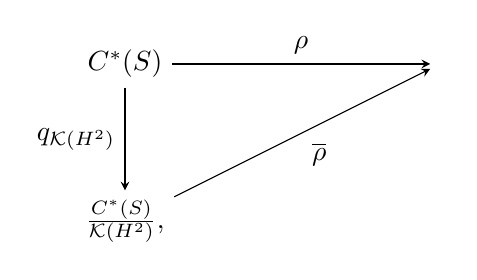
\begin{tikzpicture}[>=stealth, node distance=3cm]
    
            \node (S) at (0,2) {$C^*(S)$};
            \node (A) at (4,2) {$\bh$};
            \node (Q) at (0,0) {$\frac{C^*({S})}{\mathcal{K}(H^2)}$,};
            
            % top arrow (unlabeled)
            \draw[->]  (S) -- node[above] {$\rho$} (A);
            
            % left diagonal arrow
            \draw[->] (S) -- node[left] {$q_{\mathcal{K}(H^2)}$} (Q);
            
            % right vertical arrow
            \draw[->] (Q) -- node[below right] {$\overline{\rho} $} (A);
            
        \end{tikzpicture}    
    \end{equation*}
    pri čemer je $\overline{\rho}: \quot{C^*({S})}{\mathcal{K}(H^2)} \to \bh$
    nerazcepna upodobitev za $\quot{C^*({S})}{\mathcal{K}(H^2)}$.
    
    V zgledu \ref{zgl:2.3} smo dokazali, da velja $\quot{C^*({S})}{\mathcal{K}(H^2)} \cong C(\T)$,
    zato je $\mathcal{H} = \C$ in $\overline{\rho} = \ev_\lambda: C(\T) \to \C$ za nek $\lambda \in \T$.
    S tem smo pokazali, da so vse robne upodobitve oblike 
    $$\rho_\lambda: C^*(S) \to \C,\quad \rho_\lambda(T_f + K) = f(\lambda).$$ 
    Dokazati moramo še, da so vse takšne upodobitve $\rho_\lambda$ res robne za $\mathcal{T}(C(\T))$.
    
    Vzemimo poljuben $\lambda \in \T$. Po izreku \ref{izr:2.4} mora obstajati neka robna upodobitev $\rho_\xi$ za $\xi \in \T$, tako da je
    $$\| \rho_\xi (T_{z + \lambda})\| = \| z + \lambda\| = 2.$$
    Ker pa funkcija $z + \lambda \in C(\T)$ zavzame svoj maksimum natanko v $z = \lambda$,
    mora veljati $\xi = \lambda$ in zato je $\rho_\lambda = \rho_\xi$ robna upodobitev.
\end{zgled}





